% Preprint version of the NeurIPS 2026 MLxOR workshop short paper.
\documentclass{article}

\PassOptionsToPackage{numbers,sort&compress}{natbib}
\usepackage[preprint]{neurips_2026}
\workshoptitle{MLxOR}
\usepackage{amsmath,amssymb,amsthm,booktabs,graphicx,microtype,url}
\graphicspath{{../results/figures/}}

% hyperref last, after natbib (loaded by neurips_2026) and amsthm, and before
% \newtheorem so the proposition gets a proper anchor. It is what generates the
% PDF outline: without it pdftex emits no /Outlines and stamps Creator: TeX.
% hidelinks keeps the printed appearance identical -- links are live but unboxed.
\usepackage[hidelinks,bookmarksnumbered]{hyperref}
\hypersetup{
  pdftitle={Feedback or Annealing? A Controlled Study of Adaptive State Aggregation},
  pdfauthor={Sunny Zhang},
}

\newtheorem{proposition}{Proposition}

\title{Feedback or Annealing?\\
A Controlled Study of Adaptive State Aggregation}

\author{%
  Sunny Zhang\\
  University of Toronto\\
  \texttt{ssunny.zhang@mail.utoronto.ca}
}

\newcommand{\err}{\operatorname{err}_{\infty}}
\newcommand{\R}{\textsc{Residual}}
\newcommand{\G}{\textsc{Geometric}}
\newcommand{\F}{\textsc{Fixed}}
\newcommand{\VI}{\textsc{VI}}

\begin{document}

\maketitle

\begin{abstract}
Adaptive state aggregation replaces full-state Bellman updates with cheaper
updates on groups of states with similar estimated values.  A feedback rule
anneals the group width, narrowing it as the Bellman residual shrinks, but any
gain may come from the schedule rather than the residual signal.  I separate
these effects on a 9,261-state inventory control problem.  On this instance,
the feedback widths follow a roughly geometric path.  I use the seed-0 feedback
run to match an open-loop geometric schedule, then compare the two methods
under three update mixes, 20 paired seeds, and five compute budgets.  Feedback
shows no consistent benefit.  Among budget comparisons with unadjusted 95\%
bootstrap intervals that exclude zero, its largest advantage is $0.2\%$ of the
comparison error and its largest disadvantage is $5.7\%$.  After 10,000
iterations, every interval contains zero and lies within the preplanned
$\pm0.02$ negligible range.  By contrast, at $(1,20)$, annealing reduces error
by $22.7\%$ after $10^5$ backups but increases it by $10.4\%$ after
$3\times10^6$.  Full-state value iteration meets its $10^{-10}$ stopping
tolerance in 4.20M backups; every 10,000-iteration aggregation run uses at
least 9.2M.  Evaluations should therefore compare feedback with fixed-width
and matched open-loop schedules, measure policy quality, and use several
compute budgets.
\end{abstract}

\section{Introduction}

State aggregation reduces the cost of dynamic programming by solving a smaller
approximation to a Markov decision process (MDP)
\citep{whitt1978,bertsekas1989,li2006}.  In \citet{chen2021}, states with similar
current values share a group; full-state updates alternate with cheaper updates
that sample one state per group.  A fixed group width $\varepsilon$ trades cost
against accuracy: wide groups are cheaper, while narrow groups reduce
approximation error.

The Bellman residual measures the change from another full update.  It suggests
using wide groups when estimates are changing rapidly and narrower groups as
they stabilize.  I call this gradual narrowing annealing.  However, comparison
with a fixed width cannot distinguish the value of the residual signal from the
value of annealing.

I compare feedback with a geometric schedule matched to the seed-0 feedback
run.  Once matched, the schedule is fixed and never reads the residual.  At
each update mix, it uses the same starting width, minimum width, and number of
cycles to that minimum.  The observed paths motivate the geometric comparison,
while
Proposition~\ref{prop:bound} states the contraction result that applies within
consecutive full-state sweeps.  Across five budgets, feedback adds no
consistent benefit.  Annealing has a larger effect, and its direction changes
with the compute budget.

\section{Related work}

Classical aggregation assigns one value to each state group; its errors depend
on within-group value variation \citep{whitt1978,vanroy2006,li2006}.  Adaptive
methods group by residual size \citep{bertsekas1989}, adjust partial membership
\citep{singh1995}, divide regions using value, policy, influence, or variance
\citep{munos2002}, or divide them as the value function changes
\citep{forghieri2024}.  I use \citet{chen2021}, which groups states by current
value and has asymptotic error bound $2\varepsilon/(1-\gamma)$.

Residuals give error bounds \citep{williams1993}, have been minimized directly
\citep{arruda2011}, and guide state selection in prioritized sweeping
\citep{moore1993,wingate2005}.  Because a small residual need not imply a good
policy \citep{geist2017}, I also measure policy loss.  Here the residual range
changes only group width, not membership rules, state priorities, or the
fitting objective; I do not propose a new representation or convergence
theorem.

\section{Method}
\label{sec:method}

For a finite discounted cost MDP, the Bellman update $T$ maps the current value
function $V$ to
\begin{equation}
 (TV)(s)=\min_a\left[c(s,a)+\gamma\sum_{s'}P(s'\mid s,a)V(s')\right].
 \label{eq:bellman}
\end{equation}
The solver groups values $V(s)$ into nonempty intervals of width
$\varepsilon$.  A full-state iteration evaluates \eqref{eq:bellman} for every
state.  A grouped iteration samples one state from each group, evaluates one
Bellman update for that state, and uses the result to update the shared group
value with step size $\alpha_t=1/\sqrt{t}$, where $t$ counts grouped updates.  A schedule
$(\ell_g,\ell_a)$ repeats $\ell_g$ full-state iterations followed by $\ell_a$
grouped iterations.  The groups are rebuilt before each grouped phase.  Their
values are copied back to individual states before the next full-state phase.

After each full-state sweep, I record the residual range
$r_t=\max_s(TV_t-V_t)(s)-
\min_s(TV_t-V_t)(s)$.  The tested feedback rule is
\begin{equation}
 \varepsilon_t^{\R}=\max\{\varepsilon_{\min},c r_t\},
 \qquad c=0.084,\quad \varepsilon_{\min}=0.05.
 \label{eq:residual}
\end{equation}
The choice $c=0.084$ does not use an outcome from a stochastic grouped update.
At the preplanned $(2,5)$ mix, the first grouped phase follows two common
full-state sweeps.  They give $r=5.93429$ deterministically, so
$0.084r=0.49848\approx0.5$, matching the coarsest fixed baseline.  The initial
width is therefore known before the first grouped update.  It changes with
$\ell_g$, giving
$\varepsilon^{\R}_0=0.400$, $0.499$, and $0.538$ at $(5,2)$, $(2,5)$, and
$(1,20)$.  The main control never reads $r_t$:
\begin{equation}
 \varepsilon_j^{\G}=\max\!\left\{\varepsilon_{\min},
 \varepsilon^{\R}_0\left(\frac{\varepsilon_{\min}}{\varepsilon^{\R}_0}
 \right)^{j/(C-1)}\right\},
 \label{eq:geometric}
\end{equation}
over grouped phases $j$, with $(\varepsilon^{\R}_0,C)$ set per mix to
$(0.400,7)$, $(0.499,13)$, and $(0.538,14)$: the starting width, the minimum, and
the cycle at which the seed-0 \R{} run reaches the minimum.  Once these values
are set, \G{} follows the same schedule for all 20 seeds and never reads the
residual.  In contrast, \R{} uses the residual to choose each width.  A method
with fixed $\varepsilon=0.05$ tests whether annealing is useful at all.  The
repository in Appendix~\ref{app:artifact} provides additional controls and
complete intervals.

\paragraph{Study design.}
Before running the experiment, I specified the $(2,5)$ mix, $c=0.084$, the
20\,ms primary comparison, the $\pm0.02$ equivalence range, and two geometric
controls starting at $0.4985$.  Their durations were $C=14$ for the main
control and $C=1{,}429$ for a slow control.  I call these choices preplanned.  I
later added the $(5,2)$ and $(1,20)$ mixes, the fixed-backup budget ladder, and
the matched geometric control used in Tables~\ref{tab:final}
and~\ref{tab:anytime}.  For this matched control, I take $C$ at each mix from
the seed-0 \R{} run.  At $(2,5)$ it differs from the main preplanned control by
one cycle.  Section~\ref{sec:isolates} shows what happens when the preplanned
parameters are copied to the added mixes.

\paragraph{Why use a geometric comparison?}
The observed feedback paths are close to geometric.  A standard result explains
the decay within each uninterrupted block of full-state sweeps, but does not
determine the rate across the intervening grouped phases.

\begin{proposition}[consecutive full-sweep contraction, \citealp{puterman1994}, §6.6]
\label{prop:bound}
If two full-state sweeps are consecutive, their residual ranges satisfy
$r_{t+1}\le\gamma r_t$.
\end{proposition}

This contraction result is standard \citep[][§6.6]{puterman1994}; I do not
claim it as new.  Appendix~\ref{app:proof} includes the proof to make the
constants explicit.  Grouped phases can increase the residual, so the
proposition gives no contraction bound across a complete alternating cycle and
does not predict $C$.  In this experiment, geometric fits to the feedback widths have
per-cycle factors $0.698$, $0.829$, and $0.829$ at the three mixes.  This
observation motivates the open-loop control; the exact pilot duration $C$ is
measured rather than derived from contraction.

\paragraph{Inventory MDP, protocol, and metrics.}
A state is the inventory vector $q\in\{-10,\ldots,10\}^3$, giving
$|\mathcal S|=21^3=9{,}261$.  Five choices of quote aggressiveness trade fill
probability against spread, and the one-period cost combines spread revenue with
correlated inventory risk (Appendix~\ref{app:mdp}).  I use $\gamma=0.95$ and
rescale costs so $\lVert V^*\rVert_\infty=100$.  This is a small
market-making-style control model, not a calibrated market simulator.  Each
method runs for 10,000 iterations at each mix.  The MDP instance is fixed, so
seeds $0$--$19$ vary only which state is sampled within each group.  The same
seeds are used for all methods.  The main accuracy measure is
$\err=\lVert V-V^*\rVert_\infty$, the largest absolute error across states.  I
also evaluate the policy chosen from $V$ using
$\lVert V^{\pi_V}-V^*\rVert_\infty$.
Plots against computation use counted Bellman backups.  Each full-state sweep
counts $|\mathcal S|$ backups, and each grouped sweep $t$ counts $K_t$, the number of
occupied groups.  This count favors aggregation because it omits the residual
scan and the $|\mathcal S|$ state operations for each partition rebuild and
group-to-state expansion.
Paired differences are summarized by their median and a 95\% percentile
bootstrap interval based on 10,000 resamples.  The intervals for the added
budget ladder are not adjusted for multiple comparisons.

\section{Results}

Once the residual and geometric rules reach $\varepsilon_{\min}$ their
error curves are visually indistinguishable at every mix
(Figure~\ref{fig:curves}, Appendix~\ref{app:curves}).
Table~\ref{tab:final} shows the small numerical differences.  At all three
mixes, the 95\% interval for residual minus matched geometric both contains zero
and stays within $\pm0.02$.  The median differences are $1.7\times10^{-7}$,
$5.1\times10^{-7}$, and $-0.00201$.  Thus, when the comparison has the same
starting width, minimum width, and time to that minimum, using the residual does
not improve the result after 10,000 iterations.

\begin{table}[b]
  \centering
  \scriptsize
  \setlength{\tabcolsep}{3.0pt}
  \caption{Results after 10,000 iterations over 20 paired seeds.  R/G/F denote
  residual, matched geometric, and fixed $\varepsilon=0.05$; the policy-loss
  and backup columns use the same order.  Backups are reported in millions.
  The interval summarizes within-seed differences.}
  \label{tab:final}
  \begin{tabular}{@{}lrrrrll@{}}
    \toprule
    Mix & $\err(\mathrm R)$ & $\err(\mathrm G)$ & $\err(\mathrm F)$ & R$-$G (95\% CI)
      & Policy loss R/G/F & Backups (M) R/G/F \\
    \midrule
    $(5,2)$  & 0.05001 & 0.05001 & 0.05001
      & $1.7{\times}10^{-7}$ [$-2.8{\times}10^{-7}$, $9.0{\times}10^{-7}$]
      & 0.00210/0.00210/0.00210 & 67.685/67.684/67.686 \\
    $(2,5)$  & 0.13882 & 0.13882 & 0.13792
      & $5.1{\times}10^{-7}$ [$-9.6{\times}10^{-5}$, $2.0{\times}10^{-5}$]
      & 0.01518/0.01280/0.01280 & 30.214/30.206/30.195 \\
    $(1,20)$ & 0.20343 & 0.20115 & 0.19093
      & $-0.00201$ [$-0.00320$, $0.00541$]
      & 0.05178/0.05178/0.01649 & 9.185/9.186/9.196 \\
    \bottomrule
  \end{tabular}
\end{table}

Value error and policy quality need not agree.  At $(2,5)$, the residual and
matched geometric methods have nearly identical value error.  Their paired
policy-loss difference is $1.2\times10^{-6}$, with a 95\% CI of
$[-0.000197,0.00251]$, so the interval contains zero.  At $(1,20)$, the residual method is worse
than fixed-$0.05$ on both measures: its value error is $0.01250$ higher
(95\% CI $[0.00745,0.01561]$), and its policy loss is $0.03529$ higher
($[0.03350,0.03748]$).  Feedback does not help on either measure here.  Within each mix, the
median computation at the end differs by at most $0.13\%$.  For the residual
method, rebuilding and expanding groups adds state operations equal to
39--96\% of its counted-backup total.  Full-state \VI{} reaches its $10^{-10}$
stopping tolerance in 454 sweeps, or 4.20M counted backups.  Each
10,000-iteration aggregation run uses 9.2--67.7M counted backups.  Aggregation
is therefore not competitive on this example;
the experiment studies one approximation method rather than proposing a better
solver.

\begin{table}[t]
  \centering
  \small
  \caption{Median paired value-error difference at fixed budgets, as a
  percentage of the comparison error; negative favors the first method.
  \G{}$-$\F{} isolates annealing and \R{}$-$\G{} the added effect of
  feedback.  $^\ast$ marks a nominal 95\% bootstrap interval excluding zero;
  intervals are not multiplicity-adjusted.  Details are in
  Appendix~\ref{app:anytime}.}
  \label{tab:anytime}
  \scriptsize
  \begin{tabular}{@{}llrrrrr@{}}
    \toprule
    Mix & Contrast & $10^5$ & $3{\times}10^5$ & $10^6$ & $3{\times}10^6$ & final \\
    \midrule
    $(5,2)$  & \G{}$-$\F{} & $-0.0$  & $-5.5^\ast$   & $+0.1^\ast$   & $-8.3^\ast$   & $-0.0$ \\
    $(5,2)$  & \R{}$-$\G{} & $+0.1$  & $+0.0$        & $-0.2^\ast$   & $+0.0$        & $+0.0$ \\
    $(2,5)$  & \G{}$-$\F{} & $-2.2^\ast$  & $-8.2^\ast$  & $+6.0^\ast$  & $-6.5^\ast$   & $+0.6^\ast$ \\
    $(2,5)$  & \R{}$-$\G{} & $+0.0$  & $+1.6^\ast$   & $-0.0$        & $+0.0$        & $+0.0$ \\
    $(1,20)$ & \G{}$-$\F{} & $-22.7^\ast$ & $-14.5^\ast$ & $-8.7^\ast$ & $+10.4^\ast$ & $+5.4^\ast$ \\
    $(1,20)$ & \R{}$-$\G{} & $+3.6^\ast$  & $+5.7^\ast$ & $+3.9^\ast$ & $-0.4$      & $-1.0$ \\
    \bottomrule
  \end{tabular}
\end{table}

\paragraph{Separating annealing from feedback.}
Results after 10,000 iterations hide annealing because each scheduled
method has used $\varepsilon_{\min}$ for most of the run; at $(5,2)$, residual
and fixed end only $3.8\times10^{-8}$ apart.  Table~\ref{tab:anytime} instead
compares four earlier budgets while widths still change.  It reports relative
differences because a $\pm0.02$ threshold is uninformative when errors are near
$10$.

Looking only at unadjusted intervals that exclude zero, feedback's largest
advantage is $0.2\%$ of the comparison error and its largest disadvantage is
$5.7\%$.  Annealing changes error by about $23\%$: at $(1,20)$ matched geometric is
$22.7\%$ better than a fixed width after $10^5$ backups but $10.4\%$ worse after
$3\times10^6$.  The schedule changes both the result and its direction, while
feedback adds no consistent benefit.  Large
differences occur during rapid error reduction; exact percentages depend on
which completed update the budget reaches.

\paragraph{The timing-based primary measure was inconclusive.}
At the preplanned 20\,ms endpoint, the $(2,5)$ comparison gave a
residual-minus-preplanned-geometric median of $-0.0417$ with 95\% CI
$[-0.0459,0.0011]$,
which is inconclusive under the specified equivalence rule.  Repeated runs
selected different iterations because error was falling rapidly and machine
load varied.

\section{What the negative result shows}
\label{sec:isolates}

\paragraph{The schedules must be matched on the right scale.}
A preplanned comparison must use the unit that triggers width changes, here
grouped phases rather than total iterations.  Copied unchanged to $(1,20)$, the
slow geometric schedule never reaches its minimum and ends ten times worse;
correcting only its cycle count removes the difference
(Appendix~\ref{app:slow}).

\paragraph{A mismatched schedule creates an apparent effect.}
Fixed at $(0.4985,14)$ for every mix, the main preplanned geometric control
differs from residual at $(5,2)$ by $0.00632$, 95\% CI
$[0.006319,0.006327]$, with all 20 seeds favoring geometric.  The mismatch causes
this precise difference: geometric starts $25\%$ wider and takes twice as long
to reach the minimum.  Matching both features reduces the difference to
$1.7\times10^{-7}$, with an interval containing zero.  Low simulation variance
can therefore make a mismatched comparison look like a feedback effect.

\section{Limitations and conclusion}

One deterministic instance, residual statistic, minimum width, and feedback
constant cannot support claims about other MDPs.  The backup count omits group
maintenance.  Feedback may still help when regional residuals
differ, the best minimum width is unknown, or computation ends before
refinement does.

In this experiment, residual feedback does not beat the matched geometric
schedule in any consistent way.  Annealing does matter, changing error by about
$23\%$ at one matched budget, but its effect changes sign.  Attributing an
improvement to feedback requires a preplanned schedule matched on its starting
width, minimum width, and duration, along with several compute budgets.

\clearpage
\bibliographystyle{unsrtnat}
\begin{thebibliography}{99}

\bibitem[Whitt(1978)]{whitt1978}
Ward Whitt.
\newblock Approximations of dynamic programs, I.
\newblock \emph{Mathematics of Operations Research}, 3(3):231--243, 1978.

\bibitem[Bertsekas and Castanon(1989)]{bertsekas1989}
Dimitri P. Bertsekas and David A. Castanon.
\newblock Adaptive aggregation methods for infinite horizon dynamic
  programming.
\newblock \emph{IEEE Transactions on Automatic Control}, 34(6):589--598, 1989.

\bibitem[Li et~al.(2006)Li, Walsh, and Littman]{li2006}
Lihong Li, Thomas J. Walsh, and Michael L. Littman.
\newblock Towards a unified theory of state abstraction for MDPs.
\newblock In \emph{Proceedings of the Ninth International Symposium on
  Artificial Intelligence and Mathematics}, 2006.

\bibitem[Chen et~al.(2021)Chen, Gaebler, Peng, Sun, and Ye]{chen2021}
Guanting Chen, Johann Demetrio Gaebler, Matt Peng, Chunlin Sun, and Yinyu Ye.
\newblock An adaptive state aggregation algorithm for Markov decision
  processes.
\newblock \emph{arXiv preprint arXiv:2107.11053}, 2021.

\bibitem[Puterman(1994)]{puterman1994}
Martin L. Puterman.
\newblock \emph{Markov Decision Processes: Discrete Stochastic Dynamic
  Programming}.
\newblock Wiley, New York, 1994.

\bibitem[Van Roy(2006)]{vanroy2006}
Benjamin Van Roy.
\newblock Performance loss bounds for approximate value iteration with state
  aggregation.
\newblock \emph{Mathematics of Operations Research}, 31(2):234--244, 2006.

\bibitem[Singh et~al.(1995)Singh, Jaakkola, and Jordan]{singh1995}
Satinder P. Singh, Tommi Jaakkola, and Michael I. Jordan.
\newblock Reinforcement learning with soft state aggregation.
\newblock In \emph{Advances in Neural Information Processing Systems 7}, pages
  361--368, 1995.

\bibitem[Munos and Moore(2002)]{munos2002}
R\'emi Munos and Andrew Moore.
\newblock Variable resolution discretization in optimal control.
\newblock \emph{Machine Learning}, 49(2--3):291--323, 2002.

\bibitem[Forghieri et~al.(2024)Forghieri, Castel, Hyon, and Le~Pennec]{forghieri2024}
Orso Forghieri, Hind Castel, Emmanuel Hyon, and Erwan Le~Pennec.
\newblock Progressive state space disaggregation for infinite horizon dynamic
  programming.
\newblock In \emph{Proceedings of the Thirty-Fourth International Conference on
  Automated Planning and Scheduling}, pages 221--229, 2024.

\bibitem[Williams and Baird(1993)]{williams1993}
Ronald J. Williams and Leemon C. Baird III.
\newblock Tight performance bounds on greedy policies based on imperfect value
  functions.
\newblock Technical Report NU-CCS-93-14, Northeastern University, 1993.

\bibitem[Arruda et~al.(2011)Arruda, Fragoso, and do~Val]{arruda2011}
E.~F. Arruda, M.~D. Fragoso, and J.~B.~R. do~Val.
\newblock Approximate dynamic programming via direct search in the space of
  value function approximations.
\newblock \emph{European Journal of Operational Research}, 211(2):343--351,
  2011.

\bibitem[Moore and Atkeson(1993)]{moore1993}
Andrew W. Moore and Christopher G. Atkeson.
\newblock Prioritized sweeping: Reinforcement learning with less data and less
  real time.
\newblock \emph{Machine Learning}, 13(1):103--130, 1993.

\bibitem[Wingate and Seppi(2005)]{wingate2005}
David Wingate and Kevin D. Seppi.
\newblock Prioritization methods for accelerating {MDP} solvers.
\newblock \emph{Journal of Machine Learning Research}, 6:851--881, 2005.

\bibitem[Geist et~al.(2017)Geist, Piot, and Pietquin]{geist2017}
Matthieu Geist, Bilal Piot, and Olivier Pietquin.
\newblock Is the Bellman residual a bad proxy?
\newblock In \emph{Advances in Neural Information Processing Systems 30}, pages
  3205--3214, 2017.

\end{thebibliography}

\clearpage
\appendix

\section{Proof of Proposition~\ref{prop:bound}}
\label{app:proof}

The following standard result says that the Bellman operator shrinks
differences when they are measured by their range \citep[][§6.6]{puterman1994}.
The proof is included to make the constants in the bound explicit.

Fix $V,U$ and a state $s$, and let $a^\ast$ attain the minimum in $(TU)(s)$.
Evaluating the bracket of \eqref{eq:bellman} at $a^\ast$ rather than at the
minimizer for $V$ gives
\begin{align*}
 (TV)(s)\;&\le\;c(s,a^\ast)+\gamma\sum_{s'}P(s'\mid s,a^\ast)V(s')
 \;=\;(TU)(s)+\gamma\sum_{s'}P(s'\mid s,a^\ast)(V-U)(s')\\
 &\le\;(TU)(s)+\gamma\max_{s'}(V-U)(s'),
\end{align*}
and the symmetric argument, taking $a^\ast$ to attain the minimum in $(TV)(s)$,
gives $(TV)(s)\ge(TU)(s)+\gamma\min_{s'}(V-U)(s')$.  Both bounds hold at every
$s$, so $(TV-TU)(s)$ lies in
$[\gamma\min(V-U),\,\gamma\max(V-U)]$.  Defining
$\operatorname{span}(x)=\max(x)-\min(x)$, it follows that
\begin{equation*}
 \operatorname{span}(TV-TU)\;\le\;\gamma\operatorname{span}(V-U).
\end{equation*}
During consecutive full-state sweeps $V_{t+1}=TV_t$ and
$V_{t+2}=TV_{t+1}$, so
$r_{t+1}=\operatorname{span}(TV_{t+1}-V_{t+1})
=\operatorname{span}(TV_{t+1}-TV_t)\le\gamma\operatorname{span}(V_{t+1}-V_t)
=\gamma\operatorname{span}(TV_t-V_t)=\gamma r_t$.

The proposition does not cover a grouped phase.  Such a phase copies updates
from representative states to their groups instead of applying $T$ to every
state, so it can increase the residual range.  No contraction factor can
therefore be multiplied across complete alternating cycles without additional
assumptions.  On this inventory instance, the geometric reference curve holds
empirically before the width reaches its floor for all 20 seeds at all three
mixes.

\section{Error over computation}
\label{app:curves}

\begin{figure}[h]
  \centering
  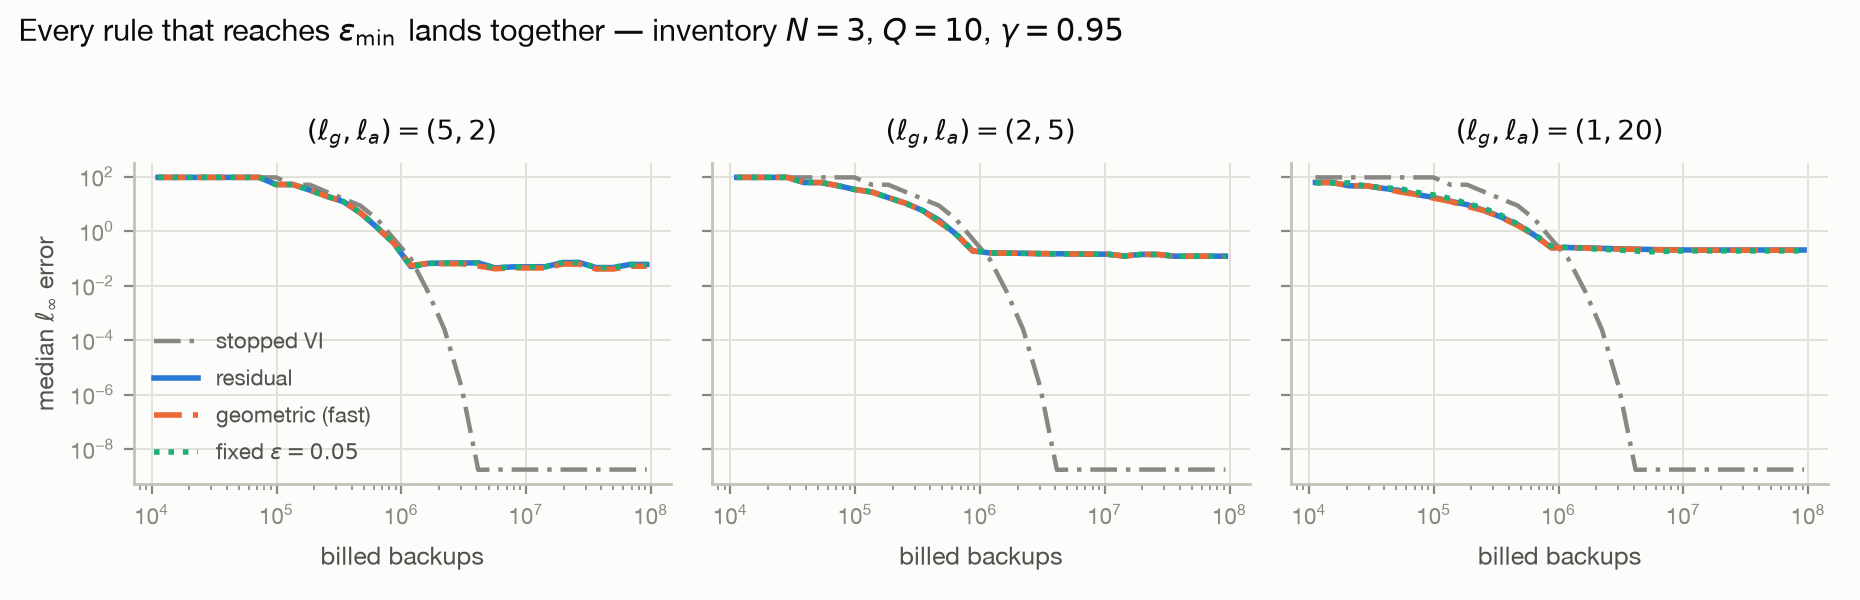
\includegraphics[width=\linewidth]{schedule_inventory_n3_light.png}
  \caption{Median value error against counted Bellman backups.  Final estimates
  are displayed beyond each method's 10,000-iteration limit.  Residual, matched
  geometric, and fixed-$0.05$ nearly coincide within each mix.  The
  deterministic \VI{} curve is repeated for reference; its convergence
  check stops after 454 sweeps (4.20M backups) though the plotted diagnostic
  continues to the common stopping point.}
  \label{fig:curves}
\end{figure}

The flat right-hand portions repeat the final values; they do not represent
continued computation.  Each method stops after $67.7$M, $30.2$M, or $9.2$M
counted backups at $(5,2)$, $(2,5)$, or $(1,20)$, respectively.  The plots
carry the last value forward so that the three panels can share an axis.
Budgets beyond a method's stopping point therefore cannot be compared fairly,
which is why the list in
Appendix~\ref{app:anytime} stops at $3\times10^6$.

\section{Inventory instance}
\label{app:mdp}

The five joint quote-aggressiveness actions have fill probabilities
$(0.1,0.2,0.4,0.6,0.8)$ and spreads $(1,0.8,0.5,0.3,0.15)$, so aggressive quotes fill
often at a worse price.  The one-period cost is
\begin{equation*}
 c(q,a)=0.02\,q^\top\Sigma q-\delta_a f_a L(q),
\end{equation*}
where $\delta_a$ and $f_a$ are the spread and fill probability of action $a$,
$\Sigma$ has unit diagonal and correlation $0.5$ so inventory risk is
correlated across the three assets, and
$L(q)=(6-\#\{i:|q_i|=10\})/6$ removes fills that would leave the box
$\{-10,\ldots,10\}^3$.  Costs are rescaled after solving so that
$\lVert V^*\rVert_\infty=100$, which puts $\varepsilon$, the equivalence
margin, and every reported error on one interpretable scale.

\section{How the budget comparisons are calculated}
\label{app:anytime}

Each cell of Table~\ref{tab:anytime} is the median over 20 seeds of the
within-seed difference divided by the comparison method's error for that seed
at the same budget.  Calculating the ratio before taking the median preserves
the pairing.  Errors are read as a step function of
counted backups: each budget uses the most recent completed update.  The list
stops at $3\times10^6$ because the cheapest mix, $(1,20)$, performs only $9.2$M
backups in total.  Later budgets would compare a repeated final value with
continued computation.  The repository artifact reports absolute differences
and 10,000-resample percentile-bootstrap intervals for both the absolute and
relative medians.

\section{Adjusting the slow schedule across update mixes}
\label{app:slow}

The slow preplanned geometric method used 1,429 grouped-update cycles, exactly the
number induced by 10,000 iterations at cycle length seven.  Transplanted
unchanged to $(1,20)$, whose cycle length is 21, it receives only 477 grouped
phases and is still narrowing at the stopping point.  It ends at
$\varepsilon=0.232$ and
error $1.59$, an order of magnitude worse than every other method.  Recalculating
only its cycle count to 477, changing nothing else, ends it at
$\varepsilon=0.05024$ and error $0.209$, back in the neighborhood of residual
and matched geometric.  The poor result came from an unfinished schedule, not
from the lack of feedback.  For this reason, the added mixes use the schedule
with the corrected cycle count.

\section{Code and result artifact}
\label{app:artifact}

The repository at
\url{https://github.com/sunnysanitize/Residual-Epsilon-Aggregation} provides
code, configurations, complete intervals, and additional controls.

\end{document}
